\subsection*{Curve-shortening flow}

\begin{frame}
{Model workflow}

\only<1>{
	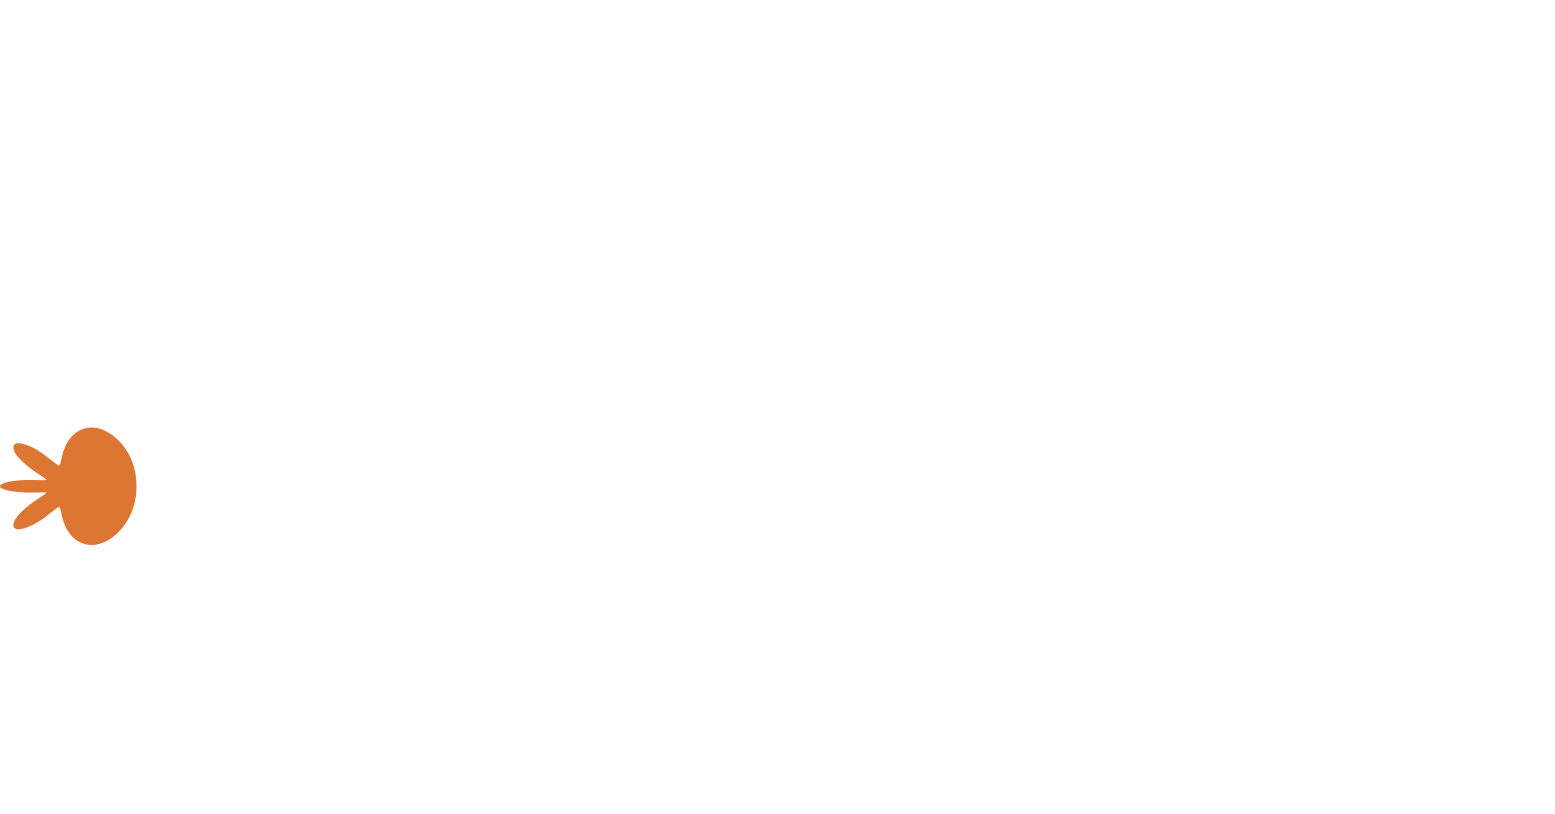
\includegraphics[scale=0.36]{figures/model-workflow/workflow-1.png}}
\only<2>{
	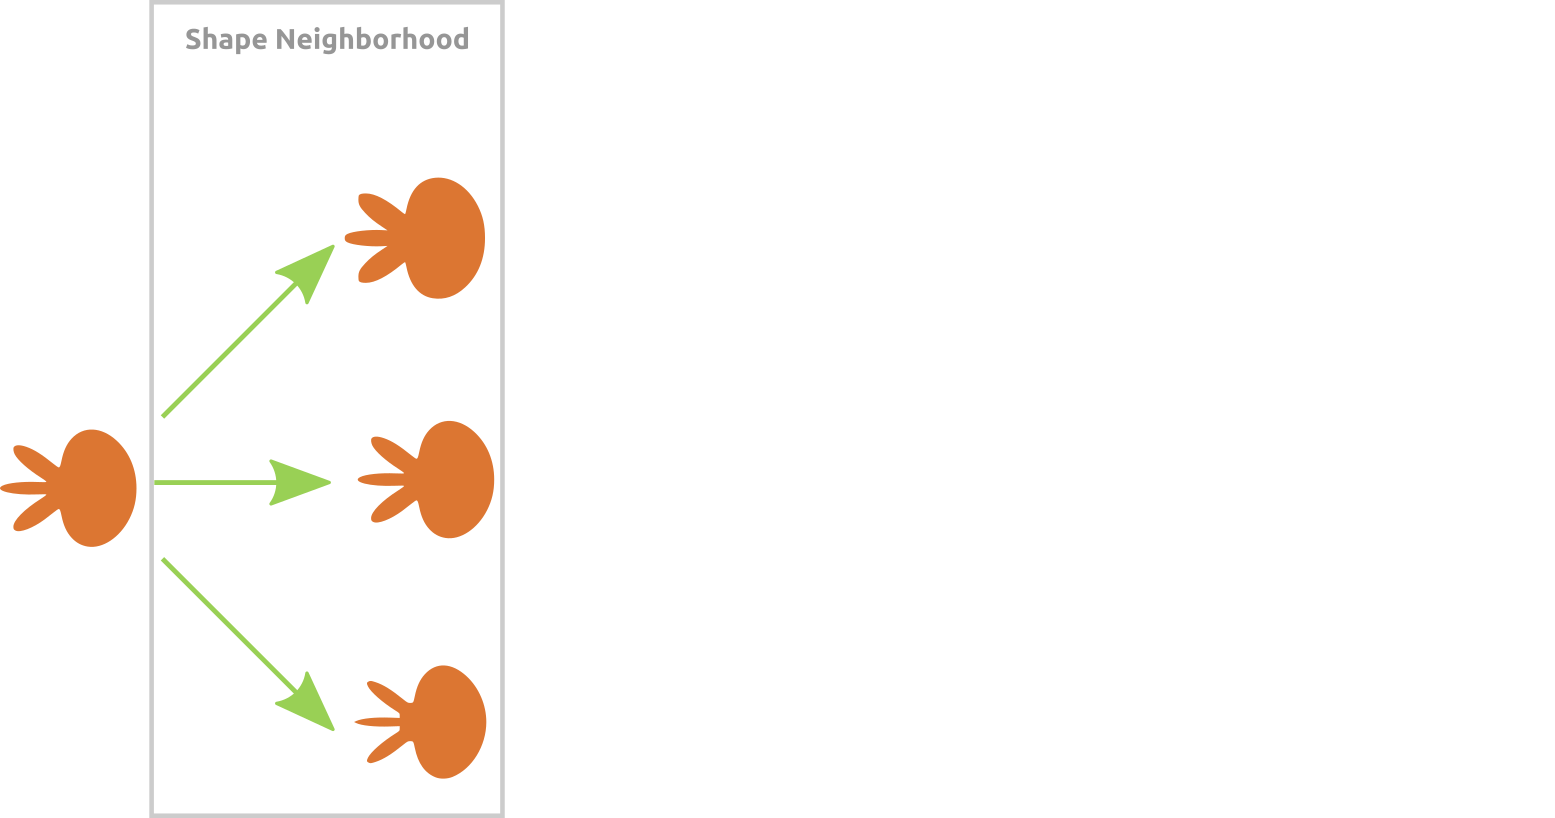
\includegraphics[scale=0.36]{figures/model-workflow/workflow-2.png}}	
\only<3>{
	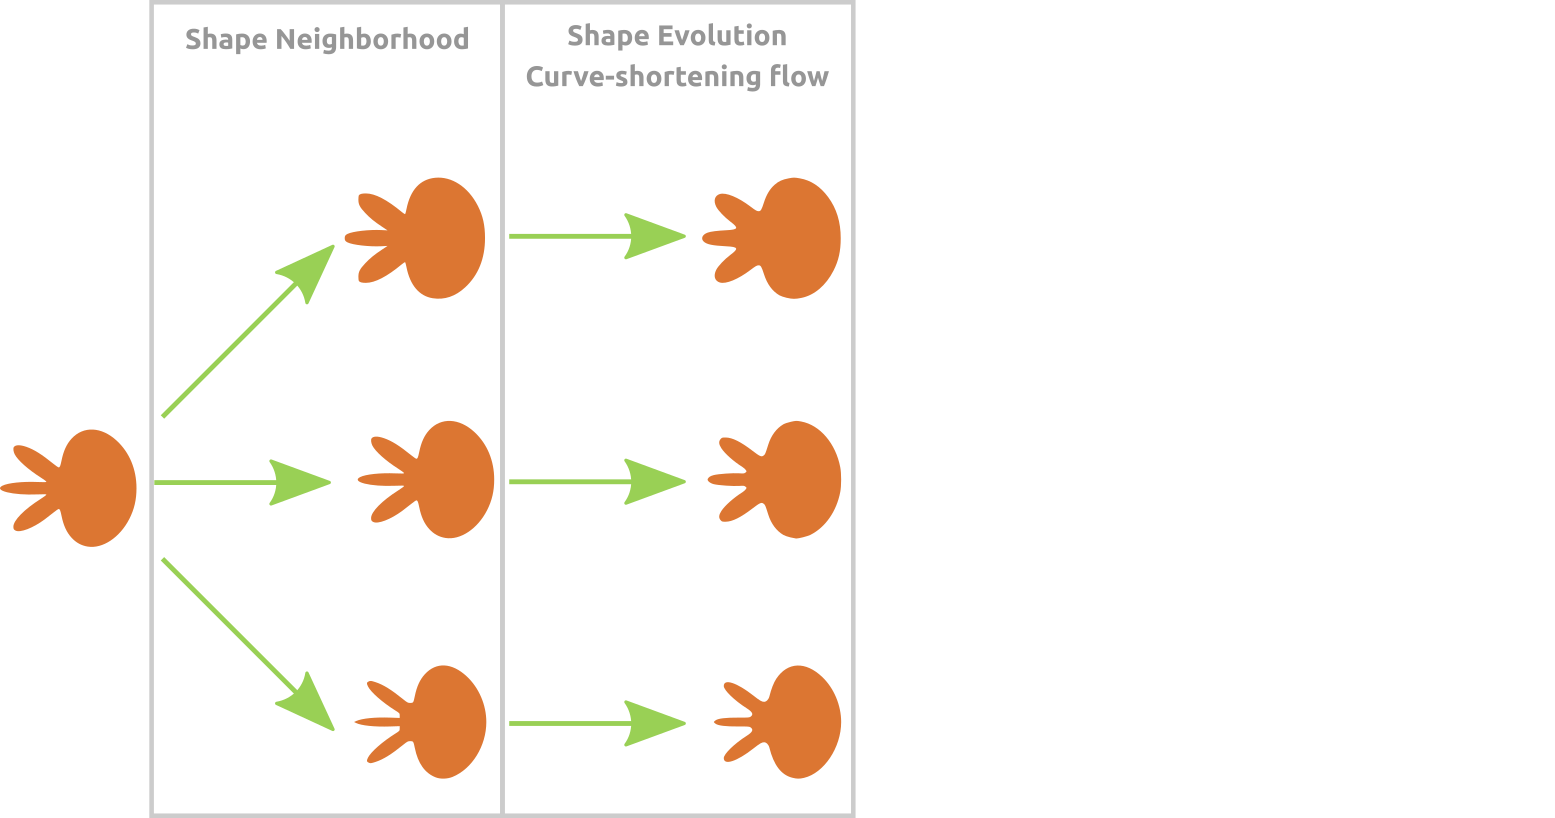
\includegraphics[scale=0.36]{figures/model-workflow/workflow-3.png}}	
\only<4>{
	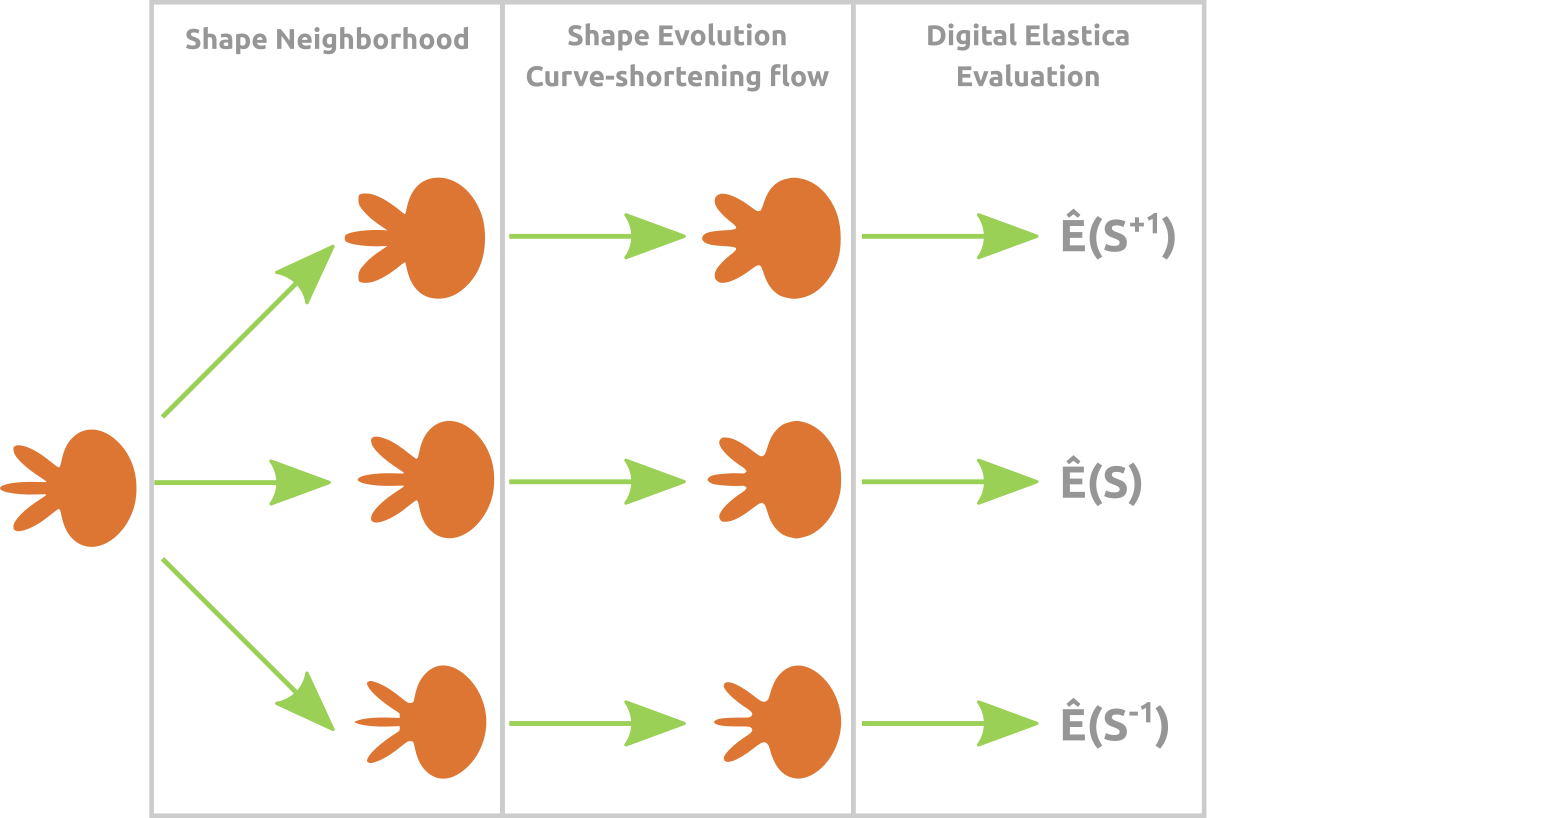
\includegraphics[scale=0.36]{figures/model-workflow/workflow-4.png}}	
\only<5>{
	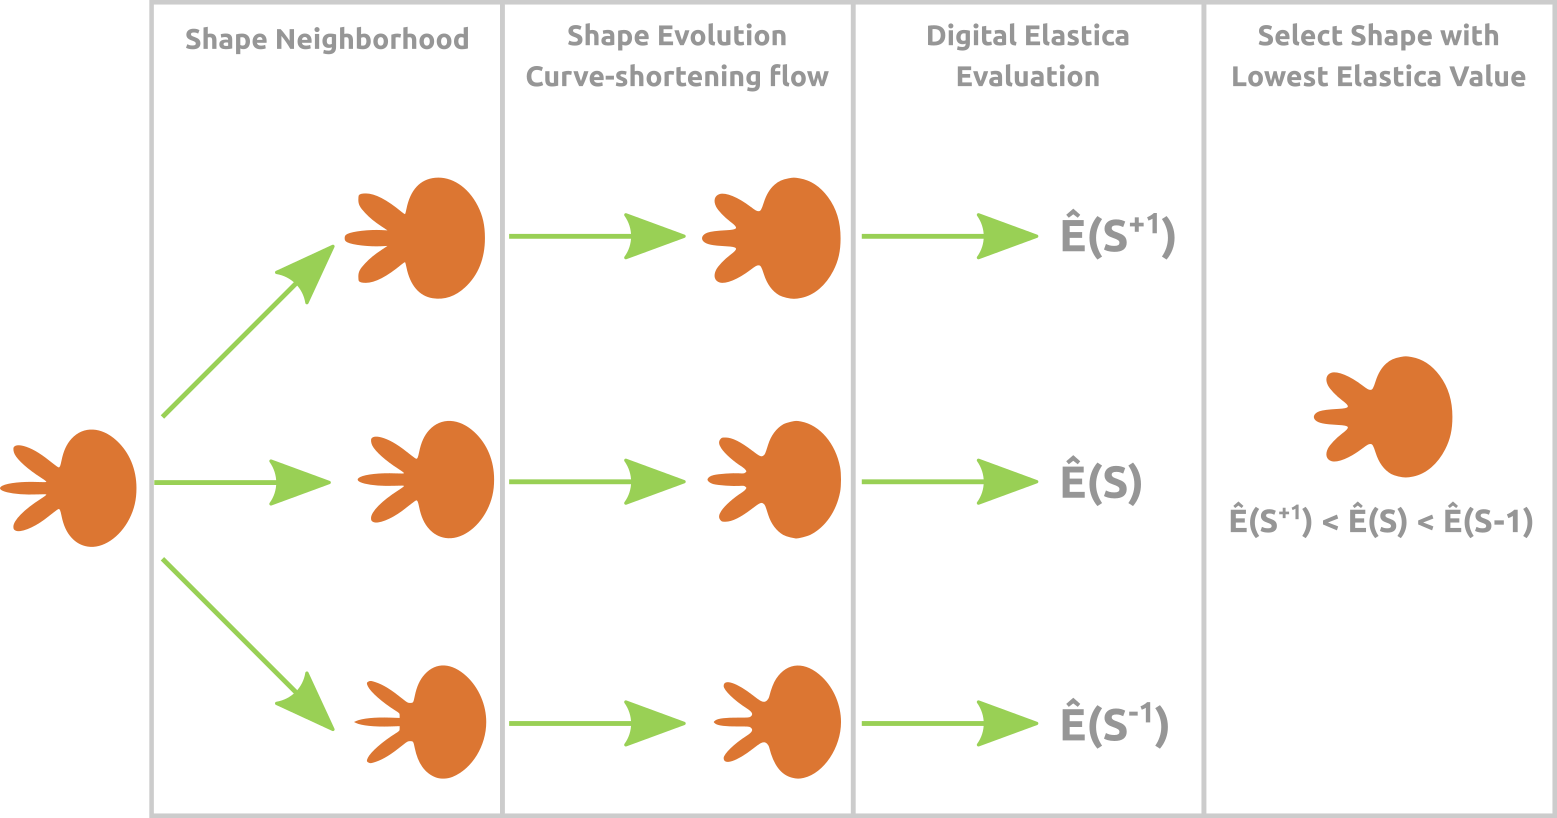
\includegraphics[scale=0.36]{figures/model-workflow/workflow-5.png}}	
\only<6>{
	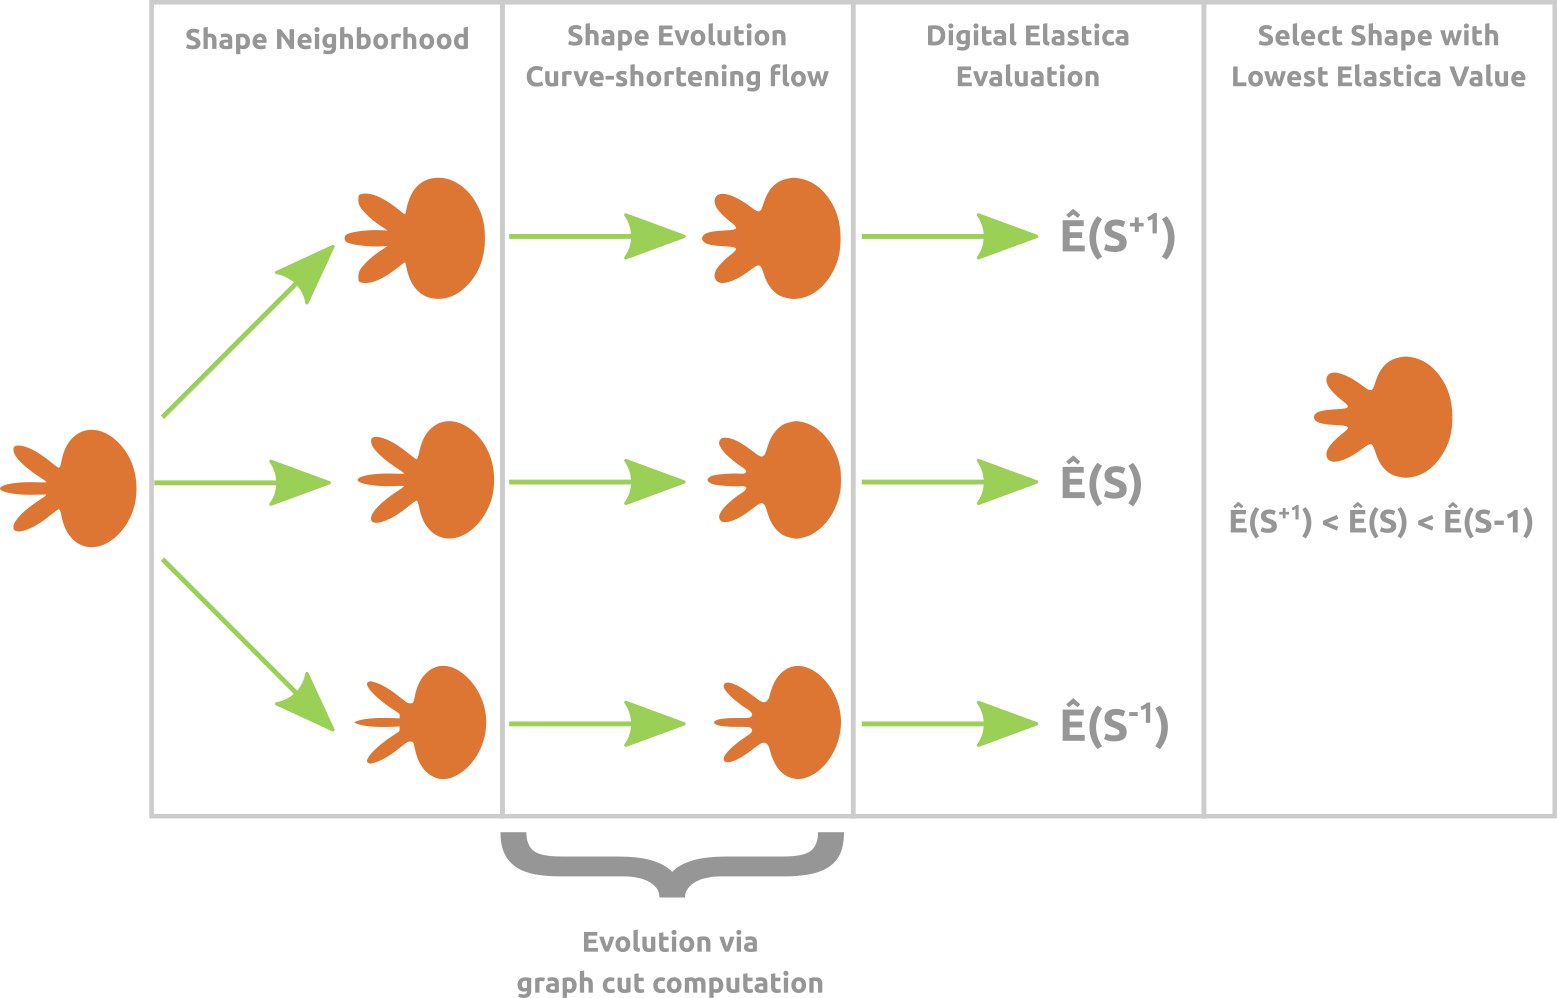
\includegraphics[scale=0.36]{figures/model-workflow/workflow-6.png}}	
\only<7>{
	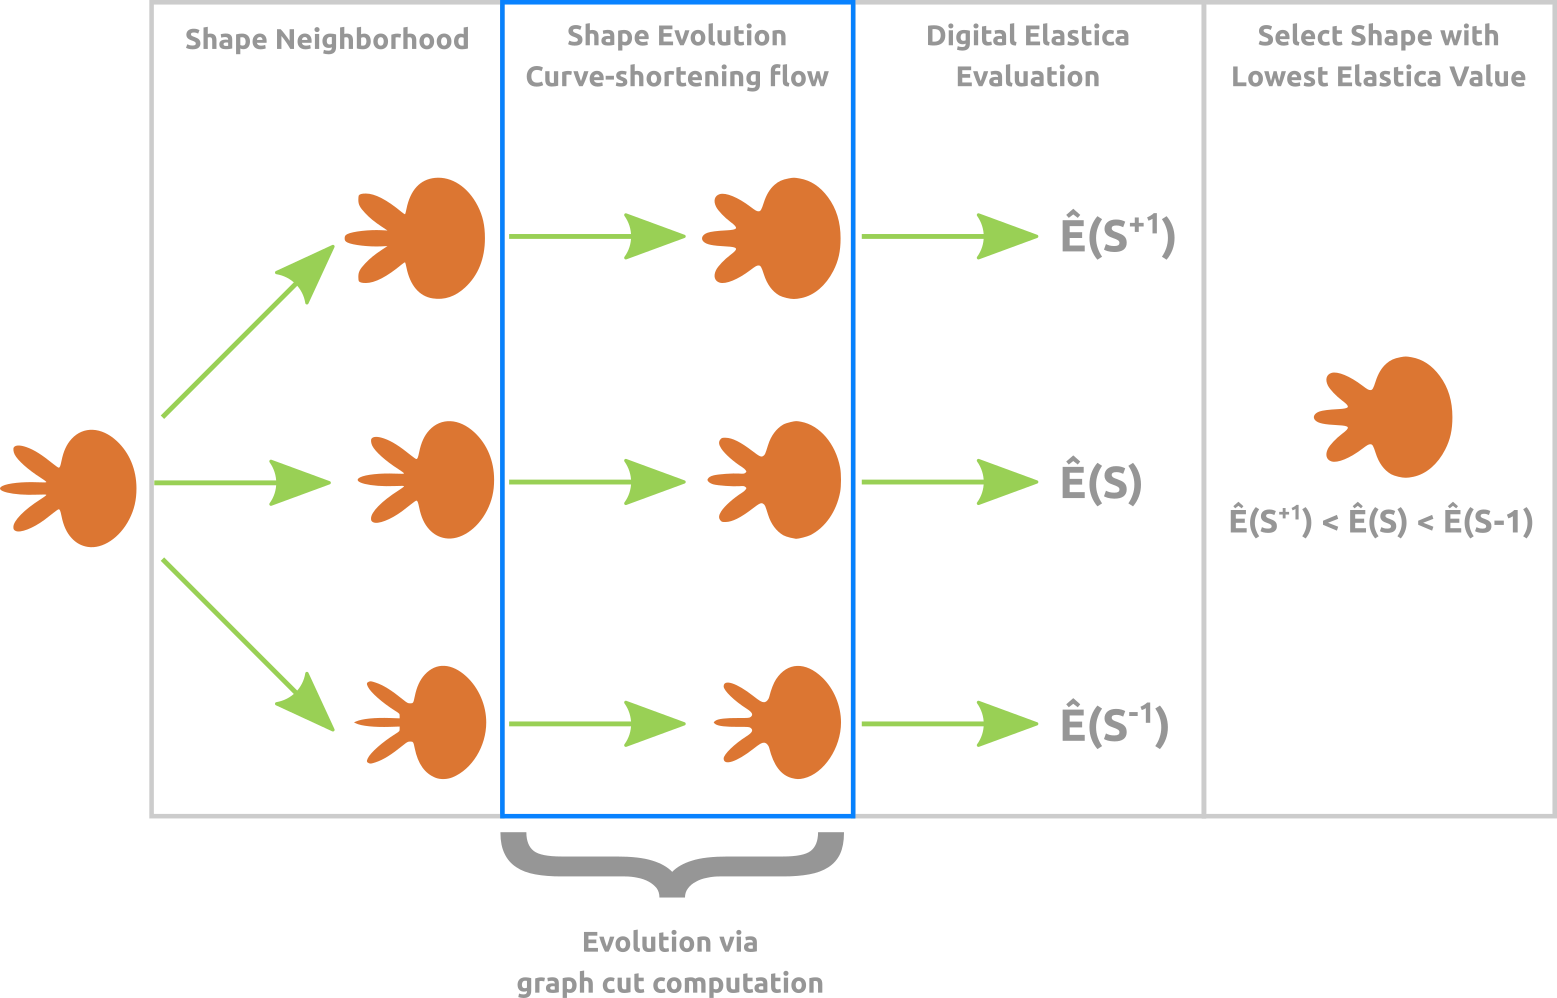
\includegraphics[scale=0.36]{figures/model-workflow/workflow-curve-shortening-flow.png}}	

\end{frame}

\begin{frame}
{Curve-shortening flow}
\begin{minipage}{0.5\textwidth}
\center
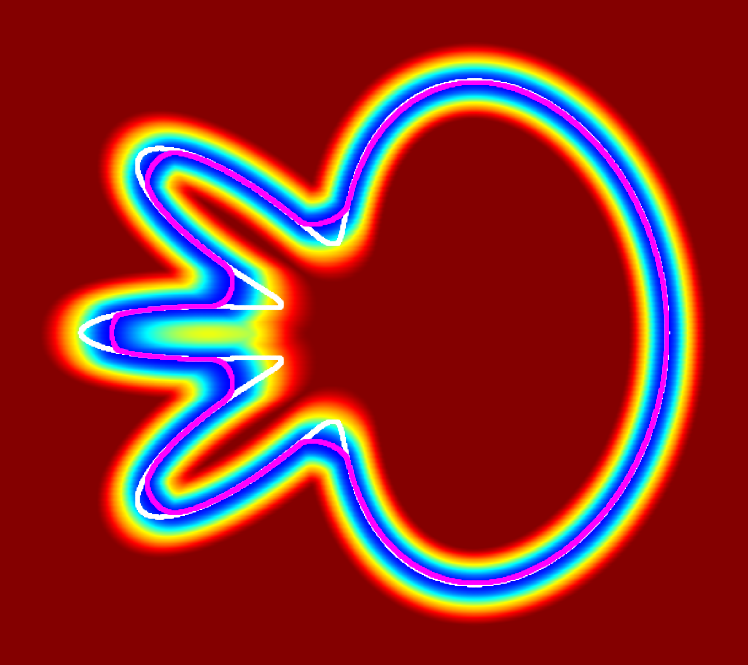
\includegraphics[scale=0.2]{figures/curve-shortening-flow/balance-coefficient-zero-level-set.png}
\end{minipage}
\begin{minipage}{0.49\textwidth}
\footnotesize
\begin{itemize}
\item{Balance coefficient}
\begin{align*}
u_r(D,p) &= \left( \frac{\pi r^2}{2} - |B_r(p) \cap D| \right)^2
\end{align*}
\item{White contour: contour of the shape}
\item{Pink contour: $\epsilon$-level set of the balance coefficient}
\end{itemize}
\end{minipage}
\end{frame}


\begin{frame}
{Curve-shortening flow}

\begin{minipage}{0.3\textwidth}
\only<1>{
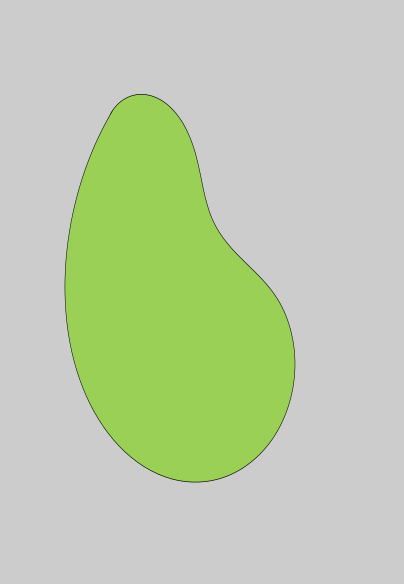
\includegraphics[scale=0.5]{figures/curve-shortening-flow/graph-model-1.png}}%
\only<2-3>{
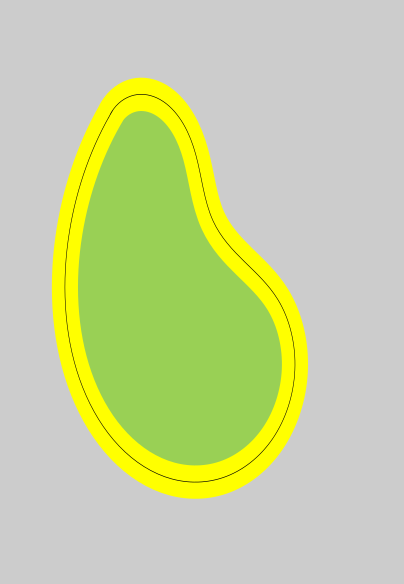
\includegraphics[scale=0.5]{figures/curve-shortening-flow/graph-model-2.png}}%
\only<4->{
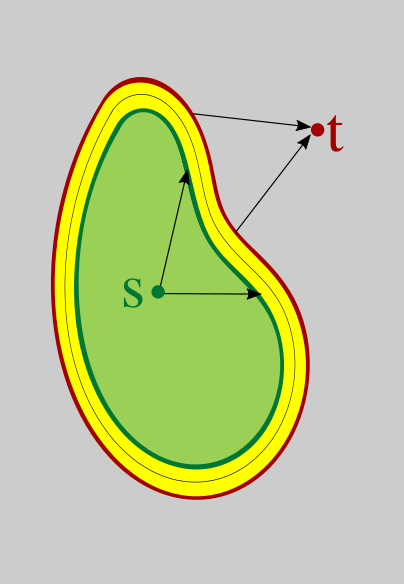
\includegraphics[scale=0.5]{figures/curve-shortening-flow/graph-model-3.png}}%
\end{minipage}
%
%
\begin{minipage}{0.69\textwidth}
\footnotesize
\begin{itemize}
\itemsep0em
\onslide<2->{\item{Optimization band
\begin{align*}
%\only<2>{O_n(D) :=& \{ p \in D \; | \; -n \leq d_D(p) \leq n \} \\}
\only<2->{O(D) :=& \{ p \in D \; | \; -n \leq d_D(p) \leq n \} \\}
\onslide<3->{F(D) :=& D \setminus O(D)}
\end{align*}}\vspace{-1em}}
\onslide<4->{\item{Graph $\mathcal{G}_D(\mathcal{V},\mathcal{E},c)$
\begin{align*}
\mathcal{V} &= \{ v_p \; | \; p \in O(D) \} \cup \{s,t\} \\
\highlight{6}{4,5,7-}{\mathcal{E}} &= \highlight{6}{4,5,7-}{\{ \{v_p,v_q\} \; | \; p,q \in O(D) \text{ and } q \in \mathcal{N}_4(p) \}} \cup \highlight{5}{4,6-}{\mathcal{E}_{st}} \\
\highlight{5}{4,6-}{\mathcal{E}_{st}} &= \highlight{5}{4,6-}{\{ (s,v_p), (v_p,t) \; | \; p \in O(D) \}}
\end{align*}}\vspace{-1em}}
\onslide<7->{\item{Edge's weight
\begin{center}
\begin{tabular}{|c|c|}
\hline
\textbf{edge} $e$ & $\mathbf{c(e)}$\\
\hline
$\{v_p, v_q\}$ & $ \frac{1}{2}\left( u_r(D,p) + u_r(D,q)\right) $\\
\hline
$(s,v_p)$ & $M$\\
\hline
$(v_p, t)$ & $M$\\
\hline
\end{tabular}
\end{center}
}}
\onslide<8->{\item{Digital shape update
\begin{align*}
D^{(k+1)} &= F(D^{(k)}) + S^{(k)}
\end{align*}}}
\end{itemize}
\end{minipage}
\end{frame}
%
%
%
\begin{frame}
{Curve-shortening flow}

\begin{center}

\begin{tabular}{cc}
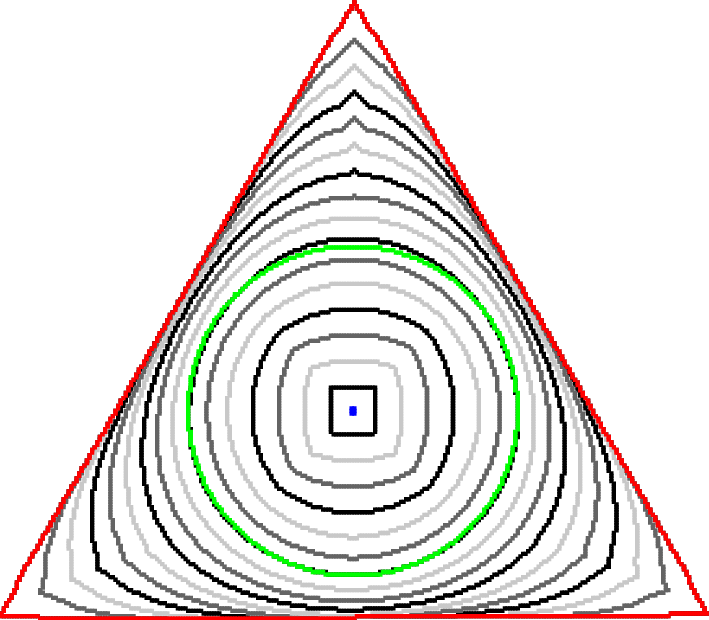
\includegraphics[scale=0.1]{figures/curve-shortening-flow/no-neighborhood-flow-always-evolve/0.015625/triangle.png}\hspace{3em} &
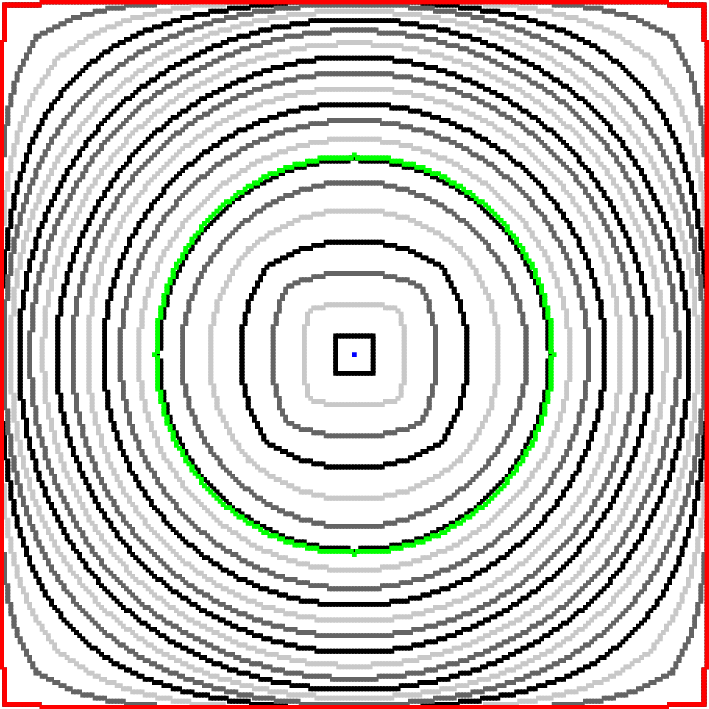
\includegraphics[scale=0.08]{figures/curve-shortening-flow/no-neighborhood-flow-always-evolve/0.015625/square.png}\\[1em]
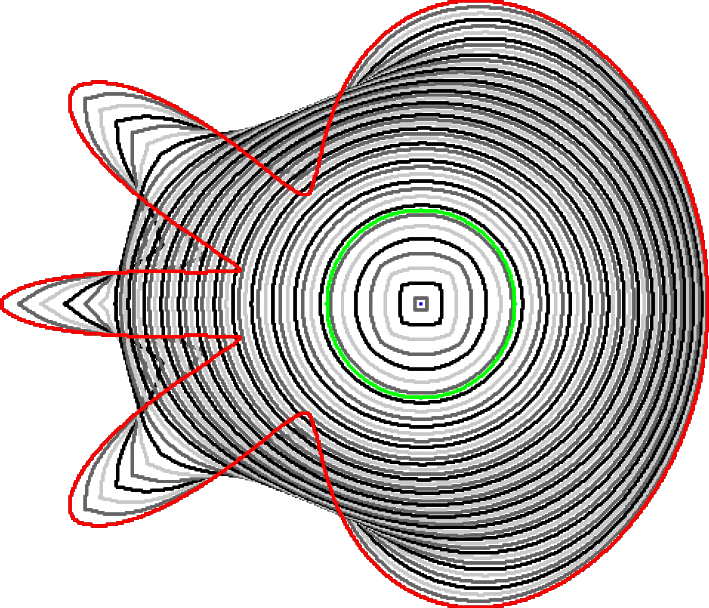
\includegraphics[scale=0.12]{figures/curve-shortening-flow/no-neighborhood-flow-always-evolve/0.015625/flower.png}\hspace{3em} &
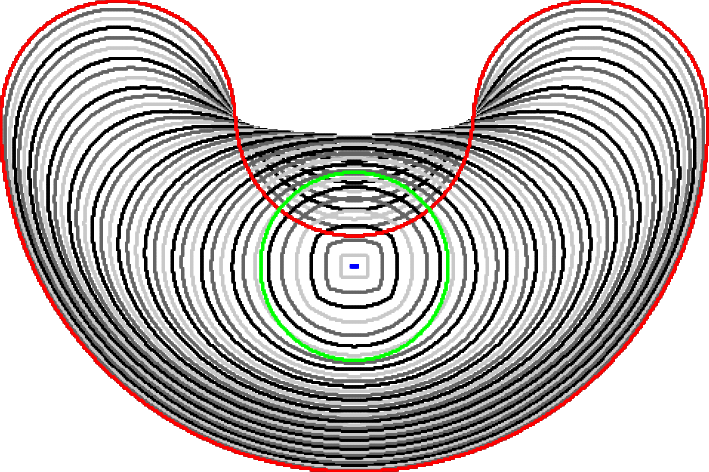
\includegraphics[scale=0.12]{figures/curve-shortening-flow/no-neighborhood-flow-always-evolve/0.015625/bean.png}
\end{tabular}
\end{center}

\end{frame}